Die zu erstellenden Prototypen erhalten die Namen \it{amilia-qouch} und \it{amilia-rdx}, wobei Amilia der Name ist, der sich in den Beispielkontakten in den Szenarien wiederfindet. Die Abkürzung \it{rdx} steht für Redux und zeigt, dass dieser Prototyp \sc{Redux Offline} verwendet. Die Endung \tt{qouch} soll die Symbiose von CouchDB und PouchDB darstellen. Der Buchstabe Q klingt wie das hart ausgesprochene C in Couch und wenn man das kleine Q horizontal spiegelt, sieht man das P für Pouch.\\\\
Beide Prototypen setzen sich aus den nachfolgend beschriebenen Komponenten zusammen, welche in \autoref{fig:uml} veranschaulicht werden. Die Abbildung stellt ein Komponentendiagramm dar. Es handelt sich hierbei nicht um das UML Komponentendiagramm, sondern um ein eigens entworfenes. Die Bezeichnung ist durch die Darstellung von React Komponenten begründet.\\\\
Jeder Kasten repräsentiert eine Komponente, deren Bezeichnung im Kopf steht.
Alle Komponenten auf der linken Seite sind View--Komponenten und können den Appstatus nicht manipulieren. Sie können nur die von der Elternkomponente durchgereichten Funktionen aufrufen.
Anhand der Linien ist abzulesen auf welche Funktionen und Eigenschaften die View--Komponenten Zugriff haben. Es werden für jede Komponente nur die eigens implementierten Funktionen aufgelistet.\\
Auf der rechten Seite stehen die Model--Komponenten. Sie manipulieren den Appstatus und entscheiden welche View--Komponente gerendert wird.
%
\begin{figure}[ht]
  \centering
  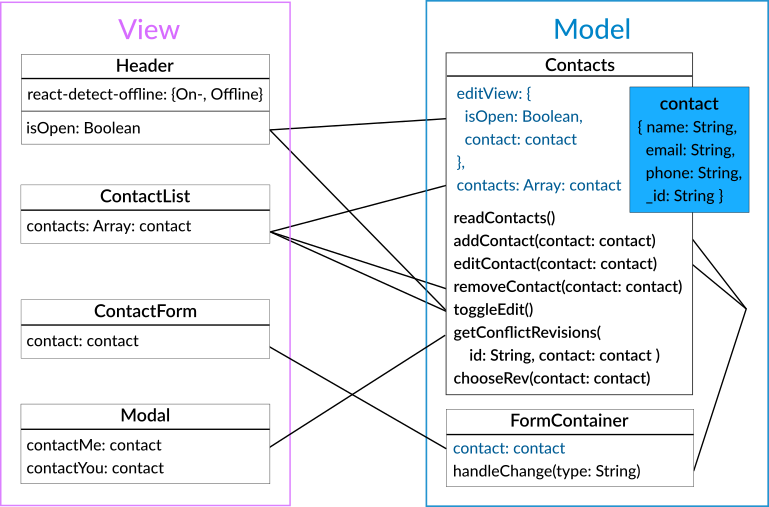
\includegraphics[width=\textwidth]{uml}
  \grayRule
  \caption[Komponentendiagramm]{Komponentendiagramm der Prototypen}
  \label{fig:uml}
\end{figure}
%
Die Komponente \tt{Contacts} fungiert als Container und ist das Herzstück der Anwendung. Er definiert die graphische Oberfläche und stellt alle notwendigen Funktionen bereit. Sie hat einen internen \tt{state} in dem sowohl die Kontaktliste, als auch die Daten für das Formular gespeichert sind. Im Diagramm ist der \tt{state} an der blauen Schrift zu erkennen.
Das Objekt \tt{editView} zeigt, welche Ansicht -- Liste oder Formular -- gerade aktuell ist und speichert den im Formular zu ladenden Kontakt.
Wie das Kontaktobjekt aufgebaut ist zeigt der blaue Kasten im Diagramm.
Wird eine Aktion zum Ändern der Ansicht aufgerufen, beispielsweise durch das Betätigen eines Knopfes, wird über die Funktion \tt{toggleEdit()} der interne \tt{state} aktualisiert und ein erneutes Rendern der Komponente eingeleitet. Dann wird entsprechend die Liste oder das Formular gerendert.\\
%
Der \tt{Header} implementiert das externe Modul \tt{react-detect-offline} und kann so den Netzwerkstatus anzeigen. Die Komponente hat Zugriff auf die \tt{toggleEdit}--Funktion und einen Knopf, der an diese gebunden ist. Damit kann das Rendern des Kontaktformulars eingeleitet werden.
Dieser Knopf soll nur angezeigt werden, wenn die Liste aktiv ist. Diese Information ist in dem  Attribut \tt{isOpen} abzulesen.\\
Die \tt{ContactList} repräsentiert die Kontaktliste und wird initial gerendert. Hier werden alle Kontakte als Liste dargestellt.
Es kann das Bearbeiten, durch den Aufruf der durchgereichten Funktion \tt{toggleEdit()} eingeleitet werden. Durch den Aufruf von \tt{remove"-Contact()} wird der Kontakt gelöscht.\\
%
Die Komponente \tt{ContactForm} zeigt, sofern vorhanden, alle im Kontakt gespeicherten Daten an.
Gibt es keine Kontaktdaten die geladen werden können, kann ein neuer Kontakt angelegt werden.
In der View, dem \tt{ContactForm} gibt es zum Hinzufügen und Bearbeiten des Kontakts Eingabefelder für den Namen, die E-Mail und die Telefonnummer des Kontakts.
Zusätzlich zu den Eingabefeldern für jedes Kontaktattribut hat sie zwei Knöpfe mit denen die Aktion bestätigt oder abgebrochen werden kann.\\
Der dazugehörige Ereignisbehandler befindet sich im \tt{FormContainer}. 
Der ''lauscht' auf die Veränderung der einzelnen Eingabefelder und speichert alle Änderungen in einer Kopie des Kontakts im internen \tt{state} '.
Wird die Aktion durch den entsprechenden Knopf bestätigt, wird die Kopie des Kontakts an \tt{Contacts} gegeben und dort entweder via \tt{addContact()} hinzugefügt, oder via \tt{editContact()} bearbeitet.
Wenn die Aktion abgebrochen wird, ruft der \tt{FormContainer} die \tt{toggleEdit()} Funktion in der Hauptkomponente auf.\\\\
%
%
Kommt es beim Hinzufügen, Bearbeiten oder Löschen eines Kontakts zum Konflikt, werden mittels \tt{getConflictRevisions()} die beiden Versionen des konfliktbehafteten Kontakts ermittelt.
Der Kontakt wird dann in beiden Varianten, der alten und der neueren Version, an einen Konfiktdialog übergeben, der sich prompt öffnet. Dieser hat Zugriff auf die Funktion \tt{chooseRev} in der \tt{Contacts} Komponente. Der Dialog hat pro Kontakt einen Knopf. Jeder dieser Knöpfe ruft auf Klick die \tt{ChooseRev} Funktion mit dem ausgewähltem Kontakt als Parameter auf.
Innerhalb von \tt{chooseRev} wird der übergebene Kontakt gespeichert und die konkurrierende Version verworfen.\\\\
%
% 
%
Eine Backendimplementierung ist für den Prototypen \it{amilia-qouch} nicht notwendig, da dies bereits durch die Verwendung von CouchDB gegeben ist.
Die \autoref{fig:qouch-model} skizziert die Architektur von \it{amilia-qouch}. Die Contacts Komponente fungiert als Model. Sie handhabt die Daten die in den View Komponenten angezeigt werden und speichert sie in der PouchDB.Die PouchDB synchronisiert sich mit der CouchDB und schreibt die Daten zurück in das Model.  
% Client - Server - Modell
\begin{figure}[H]
  \centering
  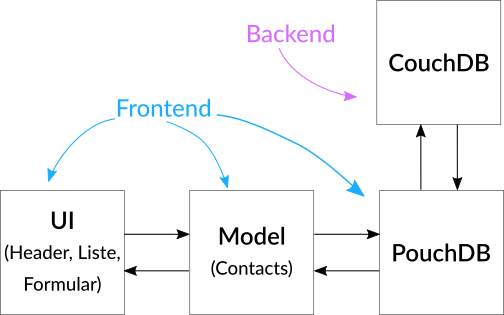
\includegraphics[width=0.8\textwidth]{qouch-model}
  \grayRule
  \caption{Client-Server-Modell des Prototypen \it{amilia-qouch}}
  \label{fig:qouch-model}
\end{figure}
%
Obwohl Redux Offline nach eigener Aussage die Datenbank ersetzt~\cite{redux-offline}, stellt es keine Serverdatenbank zur Verfügung.
Deswegen wird ein Node Server erstellt der alle \gls{CRUD} Operationen unterstützt. Die Kontakte werden in einer \gls{JSON} Datei persistiert.
Die \autoref{fig:rdx-model} zeigt sehr gut, dass der Redux Store in \it{amilia-rdx} die PouchDB \it{amilia-pouch} ersetzt.
Dabei handelt es sich um den Redux Store, der dank Redux Offline alle Daten in einer lokalen Datenbank speichert.
Die im \it{amilia-qouch} verwendete CouchDB wird von dem Server und einer \gls{JSON} Datei ersetzt.
%
\begin{figure}[ht]
  \centering
  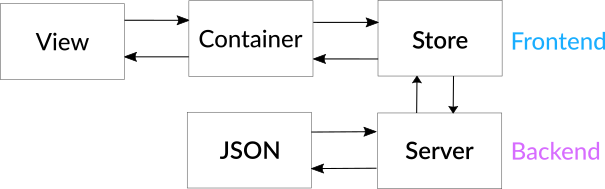
\includegraphics[width=0.8\textwidth]{rdx-model}
  \grayRule
  \caption{Client-Server-Modell des Prototypen \it{amilia-rdx}}
  \label{fig:rdx-model}
\end{figure}
% 
Der Datenfluss ist derselbe wie im Model des Prototyps \it{amilia-qouch} mit dem Unterschied, dass der Store und der Server sich nicht automatisch synchronisieren.
Der Store schickt zwar automatisch die Daten an den Server sobald er mit dem Internet verbunden ist, aber die andere Richtung ist ist das nicht implementiert.
Deswegen werden nach jeder Aktion, die Kontakte vom Server geladen.
% Todo: werden nur die geladen die es noch nicht gibt? 